\documentclass[preprint]{aastex}
\usepackage{amsmath,amssymb}
\usepackage{mathrsfs}
\usepackage{graphicx}
\usepackage{natbib}
\usepackage{bm}
\bibliographystyle{apj}

\newcommand{\mli}[1]{\mathit{#1}}
%\usepackage{epstopdf}

\begin{document}

\title{Model for DES Type Ia Supernova Cosmology Analysis}
\author{Alex Kim}

\section{Model}
We infer a Hubble diagram based on measurements of discovered transients
that have passed some selection criteria (e.g.\ classified as Type~Ia supernovae, SNe~Ia).  The probability distribution
function (pdf) of the Hubble diagram is denoted as
\begin{equation}
p({\mu},{z} |  {{ADU}}, {{T}}_S,{{z}}_S,
{{\theta}}_S;
{\text{RA}}, {\text{Dec}}, \text{Detected}, {\text{Selected}}).
\label{hd:eqn}
\end{equation}
The semicolon separates random and fixed parameters.
The set of distance moduli
and redshifts $(\mu, z)$ is the Hubble diagram.  The available information
from which the Hubble diagram is inferred include:
the transient photometry ${ADU}$; spectral measurements of
transient
type, redshift and SN-parameters ${T}_S$, ${z}_S$, ${\theta}_S$;
mass, sSFR, etc.; transient coordinates  $\text{RA}$, $\text{Dec}$;
and the fact that the transients were Detected and Selected for the analysis.

The pdf in Equation~\ref{hd:eqn} is proportional to
\begin{equation}
p({\mu},{z}; \text{RA}, \text{Dec},  \text{Detected}, {\text{Selected}}
 |  {{ADU}}, {{T}}_S,{{z}}_S,
{{\theta}}_S)
\label{hd2:eqn}
\end{equation}
and this is what we model.  A sketch of the model (with the optional inclusion
of calibration) is depicted in the Probabilistic Graphical Model
(PGM)
shown in Figure~\ref{pgm:fig}.
Note that although we have been discussing the model for the Hubble diagram, the same PGM can
 be used to express the pdf for cosmological
parameters, labelled as $\theta_\mu$.



\begin{figure}[htbp] %  figure placement: here, top, bottom, or page
   \centering
   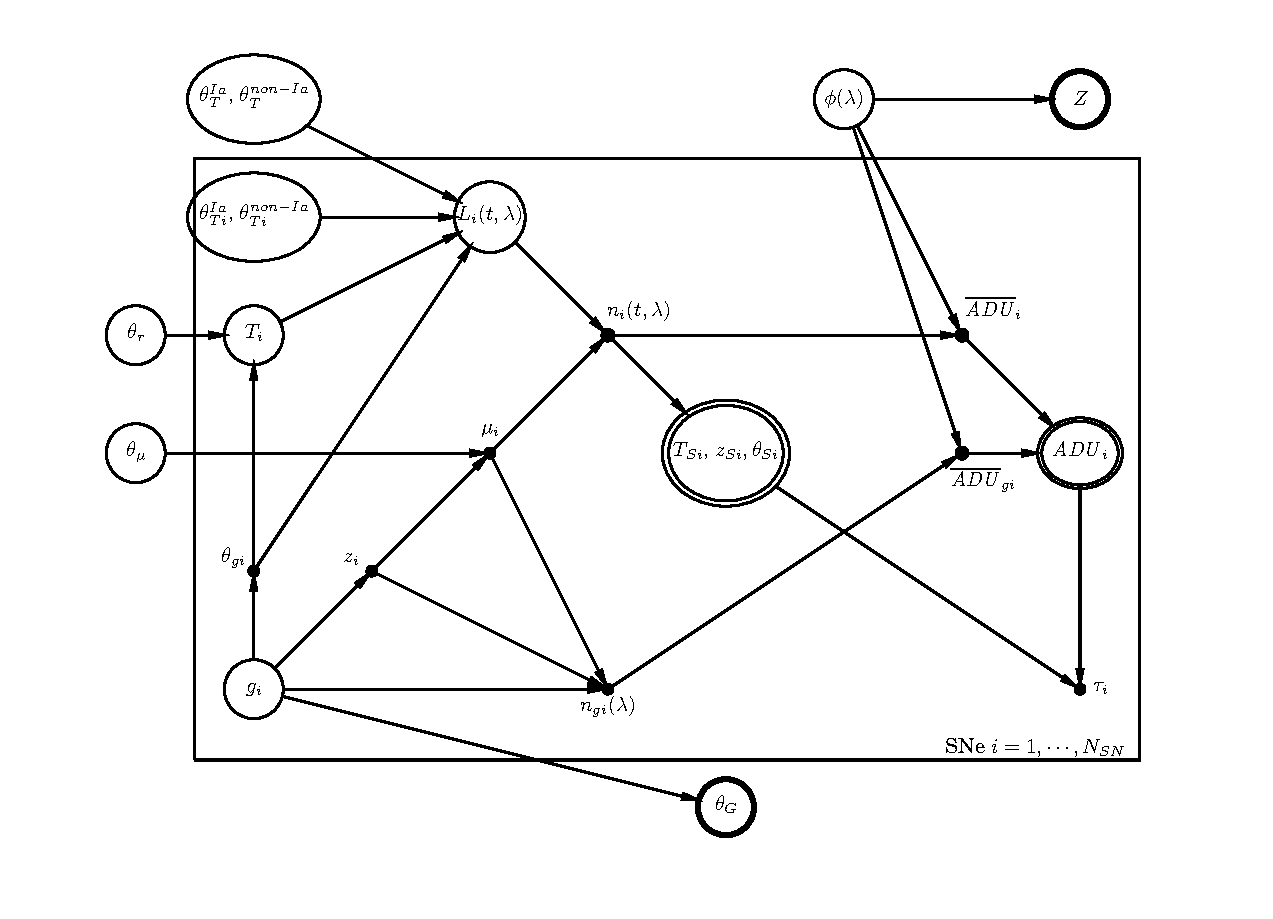
\includegraphics[width=7in]{/Users/akim/project/abc/results/hdpgm.eps} 
   \caption{Probabilistic Graphical Model for the SN~Ia analysis.  
   The forward modeling
   flow goes from left to right, starting with the description of the universe, observatory,
   and data.    A transient has
   coordinates  $\text{RA/Dec}$.  It is associated with a host host galaxy $g_i$.
   The galaxy redshift redshift $z$ and parameters $\theta_{gi}$ depend on the host.
   A distance modulus model with parameters $\theta_\mu$ fix the distance modulus $\mu_i$.
   The transient type $T$ depends on the host-galaxy.   The transient
   parameters $\theta_T^X$, $\theta_{Ti}^X$ (and perhaps the host galaxy) fix the luminosity $L$.       The 
   incoming photon flux $n$, $n_g$  are then fixed
   with redshift and distance modulus.
   The instrumental transmission function $\phi$ is calibrated with data ${Z}$ and
   gives the expected
   counts $\overline{\mathit{ADU}}$, $\overline{\mathit{ADU}}_g$. 
   The transient must be Detected and Selected and its realized light curve (${ADU}$) depends on the expected counts.  Some transients have spectral data
   ${X}_S$.
   \label{pgm:fig}}
\end{figure}


The model describes the transients that constitute the cosmology analysis, given the following
information.  
\begin{itemize}
\item ${\text{RA}}$, ${\text{Dec}}$.  The observed
coordinates.  For our purposes the observed, rather than true, coordinates are sufficient.
\item Detected.  The transient is discovered.
\item Selected. The transient is selected for the cosmology analysis.  This presumably
includes its classification as SN~Ia.
\end{itemize}

The universe is modeled as the background cosmology, transients that could
enter the sample, and their host galaxies.
\begin{itemize}
\item $P(g_i; {\text{RA}}/{\text{Dec}})$. The host galaxy $g_i$
is drawn based on coordinates.
It is drawn from
the union of the objects in the observed galaxy catalog
plus unobserved galaxies that have not
met the detection threshold, presumably due to their low surface brightness.
This pdf is
the deliverable we want from Ravi.
\item $z_i$, $\theta_{gi}$ are the galaxy redshift and parameters (e.g.\ mass, sSFR, metallicity).
For observed galaxies the parameter values are based on measurements e.g.\ $\theta_{gi} \sim \mathcal{N}({\theta}_{gi},\sigma^2_{{\theta}_{gi}})$, otherwise the distribution
of $\theta_{gi}$ for ``hostless'' galaxies is described by the model.
Redshifts may be photometric or spectroscopic.
\item $\theta_\mu$ are the parameters that specify that distance modulus.
\item $\mu_i=\mu(z_i; \theta_\mu)$.  The distance modulus is a function of redshift,
whose specific form is unspecified at the moment,  it could
be a $\Lambda$CDM prediction with cosmological parameters, a spline with knot values
as parameters.
The redshift of the galaxy is used in the Hubble diagram.
\item $P(T_i | \theta_{gi})$.  The transient type $T_i$, SN~Ia or non-Ia, depends
on the host properties.  We could make the relative rates be dependent
on specific star formation rate and morphology.
\item $p(\theta_T^{Ia}, \theta_{Ti}^{Ia})$.  The model parameters for SNe~Ia, including
parameters that describe distributions.
Different SN~Ia models could be considered: the treatment of SALT2 parameters
has been presented in \citet{2011MNRAS.418.2308M}.
The SALT2 SN~Ia
model has individual $c$ and $x_1$ parameters that would constitute $\theta_{Ti}^{Ia}$,
and global $\alpha$, $\beta$, and intrinsic dispersion  parameters  common to all supernovae
 and  underlying  $c$ and $x_1$ distributions that would constitute $\theta_T^{Ia}$.
\item $p(\theta_T^{non-Ia}, \theta_{Ti}^{non-Ia})$.  Non-Ia transients
that can be mistyped as Ia are described by a parameterized model.
\item $L_i(t,\lambda; T_i, \theta_T^{Ia}, \theta_{Ti}^{Ia}, \theta_T^{non-Ia}, \theta_{Ti}^{non-Ia},
\theta_{gi})$.  The source model fixes
the luminosity. The  model includes  information on the
source and line-of-sight effects, which specify the effective SED.   Only the
parameters of the model of the appropriate type $T$ are relevant.  The galaxy parameters
$\theta_{gi}$ are included if correlations with host-galaxy properties are to be modeled.
\item $n_i(t,\lambda; L_i, \mu_i, z_i)$, $n_{gi}(t,\lambda; L_i, \mu_i, z_i)$.  The  fluxes of
the transient and host that are incident at Earth
are fixed by the luminosity, distance modulus, and redshift.
\end{itemize}

The model expectation of measured  signals is governed by:
\begin{itemize}
\item The transmission functions $\phi(\lambda)$ describe the optical path from the
atmosphere to counts.  We expect
the calibration group to provide us with the functions and covariance,
in which case
$\phi \sim \mathcal{N}(\bar{\phi},C_\phi)$ would be a fixed condition.
\item $\overline{\mathit{ADU}}$ and
$\overline{\mathit{ADU}}_g$ are the expected counts of the transient and galaxy respectively,
coming from $\int n_i \phi d\lambda$.
\end{itemize}

The observations are as follows:
\begin{itemize}
\item ${\mathit{ADU}}$ is the realized flux can be expressed as
\begin{equation}
P({\mathit{ADU}} | \overline{\mathit{ADU}}, 
\overline{\mathit{ADU}}_g; \text{Dectected}, \text{Selected})=\frac{P({\mathit{ADU}};\text{Dectected}, \text{Selected} |  
\overline{\mathit{ADU}}, \overline{\mathit{ADU}}_g)}{P(\text{Dectected}, \text{Selected} | 
\overline{\mathit{ADU}},  \overline{{\mathit{ADU}}}_g)},
\end{equation}
which can be determined from detection and typing efficiency studies.
\item ${T}_S$, ${z}_S$, ${\theta}_S$ Transient type, redshift and properties from
spectroscopic data. I skip the details of the actual measurement  and make a direct association
with the fluxes of the transient and underlying galaxy $n$, $n_g$.
A very simple association is ${T}_S = T$, ${z}_S=z$, ${\theta}_S \in \theta_g$,
or a blurry version instead of a straight equality.
\item ${Z}$ represents the calibration measurements.   Although this may be given
by the Calibration Task Force, the PGM is written for the more general case where the calibration
is modeled within our analysis.
\end{itemize}

%
%\section{Subsections of the Model}
%
%\subsection{Type}
%\label{type:sec}
%Since our transient sample may not consist purely of SNe~Ia, the model
%has a term of the form $P(T, G | z,\mu)$, which should account for all types of
%objects that could potentially be mistaken for Type~Ia:
%the rates and association with host galaxies are described for
%the full population of potential interlopers.
%This term is not currently well known, particularly at the highest redshifts probed by DES.
%
%An idea is to consider two types: SN~Ia and non-SN~Ia, where the latter's
%intrinsic distributions have loose priors.  Transients that have been spectroscopically
%classified as non-Ia will provide the strongest leverage in constraining the
%contamination: this subset must be unbiased or properly weighted
%relative to the underlying population that constitutes the Hubble diagram.
%Running the model on a pure sample of SNe~Ia can have benefits.
%As discussed in \S\ref{systematics:sec}, comparing these results with
%those from the full sample provides
%a test of systematics.  Alternatively, the non-Ia model may be better constrained
%with the pure sample.
%
%
%To minimize the contribution of non-Ia contamination we strive for
%a pure sample selection so that $P(T=\text{non-Ia}| \mu) \rightarrow 0$.
%
%
%\subsection{Host Matching}
%\sloppy
%The host-galaxy properties depend on the GC and the transient
%coordinates $P({z}_H, {\theta}_H | {\mathit{Gals.}}, \text{RA/Dec})$.  With a
%spectrum of the transient and the underlying background, identification of the host galaxy
%is usually straightforward.
%Otherwise, projections or ambiguous cases can result in the misidentification of
%the host.
%Other supernova surveys (e.g.\ SNLS) 
%with spectroscopically confirmed host associations (e.g.\ with
%matched transient and galaxy redshifts) that replicate the DES population
%can be used to put a prior on this probability.
%
%%An effective way of addressing this term is to
%%analyze the supernovae assuming a correct host match, and
%%experimentally determine $P(\text{mismatch} )$ and
%%$\left. \langle {\mu}-\mu(z)\rangle \right|_{\text{mismatch}}$, $\left. \langle {z}-z \rangle \right|_{\text{mismatch}}$ and cross-terms to correct bias in the Hubble diagram. 
%
%
%% only model $T=\text{SN~Ia}$,
%%and experimentally determine $P(\text{non-Ia})$, 
%%$\left. \langle \mu-\mu_{model} \rangle \right|_{non-Ia}$, and its uncertainty for the
%%sample of non-Ia's that are discovered and misclassified as SN~Ia.
%%This measurement is achieved through spectroscopic
%%typing of a subset drawn from the populations used in the Hubble diagram.
%%The weighted bias would be added as a correction to the Hubble diagram under the assumption that all objects are SNe~Ia.
%
%
%
%\subsection{Type~Ia Supernova Model}
%\label{snmodel:sec}
%The DES light curve analysis in principle may be used for typing and determining
%redshift, in addition to getting supernova properties.   
%Generally the relevant term is
%\begin{equation}
%P({D}_i=1,{\mathit{ADU}}_{i}, {T}_{Si}, {z}_{Si}, {\theta}_{Si}, {z}_{Hi}, {\theta}_{Hi}
% | \mu_i,z_i,T_i,\theta_T,\theta_{Ti},\phi(\lambda)).
% \end{equation}
%Detection and typing depend on the realized light curves, and hence the truncated
%distribution of discovered transients typed as SN~Ia.
%
%The model contains a piece $P({\mathit{ADU}}_{i} {z}_{Si}| \mu_i,z_i,\theta_T, \theta_{Ti}, ,\phi(\lambda))$, which
%is the piece that describes underlying SN~Ia properties and light-curve fits.
%
%
%\subsection{Detection Efficiency}
%There term $P({D}|\mathit{ADU}_V)$.  For all high-redshift supernova searches
%I know of, this depends on the signal-to-noise of the data, and very weakly on the
%structure of the underlying galaxy.  Our detection is now based on machine learning,
%we should confirm that detection dependencies do not depend on our model parameters
%(except for RA/Dec).
%
%\section{Systematic Tests}
%\label{systematics:sec}
%The Hubble diagrams of subsets of data quantify systematic uncertainty.  
%Subsets that may be expected to show evidence for systematics include:
%spectroscopically typed SNe~Ia; transients in deep (3) versus shallow (1/2) DES fields;
%transients with NIR data; splits based on host properties.
%
%A potentially more probative test is to compare the distance moduii inferred for the same
%supernovae, but reducing the amount of data considered.  A subset of DES
%transients have higher signal-to-noise, spectroscopic confirmation, and NIR coverage than
%the average transient, we can take away that extra information in calculating distance modulus
%to get $P(\mu | \mathit{data} - \mu | \mathit{data}^-, z | \mathit{data} - z | \mathit{data}^-)$.
%It is possible that differences in $\mu$s and $z$s have smaller uncertainties that the
%$\mu$ and $z$ alone due to common measurement uncertainties. 
%
%\section{Misc.}
%DES plans a ``photometry''-only analysis, in that a significant subset of transients used
%in the Hubble diagram will not observed spectroscopically while active.  Therefore,
%our model must account for transient mistyping and host-galaxy mismatches.  To obtain
%our targeted
%accuracy we need to account for covariances that occur due to photometric
%calibration and Malmquist bias.  Our model will contain elements that may not
%have been included in previous analyses. 
%
%
%Generically ${{T}}$ can describe sample selection.  I choose to focus
%on objects typed as SN~Ia, rather than  all discovered transients, not just those typed as SN~Ia. 
%The non-Ia transient population has significant model uncertainty and the information they impart on the expansion history is weak:  I anticipate it is cleaner to limit ourselves to
%modeling discoveries we think are SN~Ia. This restriction does not obviate the need
%to consider non-Ia contamination in the sample, rather
%we only need to model non-Ia's
%that are mistaken for Ia and not all discovered transients. 
%
%
%
%Here $\mu$ is modeled; most analyses instead
%directly have cosmological parameters $\{\Omega_M, \Omega_\Lambda, w_0, w_a\}$.
%A motivation is to provide results that can be applied to test arbitrary cosmological models:
%indeed the model-dependence of the $\mu$'s reported for high-$z$ supernovae 
%\citep[e.g.][]{2012ApJ...746...85S} is a source of confusion to the community.
%%An example of a non-parametric model for $\mu$ that is independent of cosmological
%%parameters is given in the Appendix of
%%\citet{2013ApJ...764..116W}.
%
\bibliography{/Users/akim/Documents/alex}

\end{document}

